%   MSc Business Analytics Dissertation
%
%   Title:     Aaa Bbbbbbb Cccccccccc
%   Author(s): Xxxxxx Xxxxxxxxx and Yyy Yyyyyyyyy
%
%   Chapter 3: Literature Review
%
%   Change Control:
%   When     Who   Ver  What
%   -------  ----  ---  --------------------------------------------------------------
%   11Feb11  AB    0.1  Begun 
%

\chapter{Literature Review}\label{C.LitReview}
\section{Introduction}\label{S.intro3}

In recent years, purchasing capability of an \textbf{economy} has increased due to improvement in their finances, and employment levels. Ranging from buying small household items to\textbf{ expensive items such as a house, a car or an office}. To buy a house or a car, one needs to have a large amount of money available to him; that is not necessarily possible most of the time. \\

\textbf{Start with an exmaple to explain what is loan}. There are certain critical circumstances that can occur anytime, where one may need a certain amount of cash. So one may need to borrow a generous amount of money from some other entity which is called a loan. A loan is lending a sum of money from one entity to another that involves repayment of the amount in near future. Lent amount is called principal amount and amount to be repaid is a summation of principal amount and an interest amount or other charges. It is not as easy as it sounds like, there are certain terms need to be agreed upon by each entity before exchange of the money. A loan can be for an amount taken at one time or can be taken in instalments {Partial Payments]. A loan can be provided by banks, corporations and financial institutions. Banks and financial institutions provide various types of loans as per the need of an applicant, such as personal loans, home loans, business loans, credit card loans and cash advances. There are times when the borrowing amount is very large and banks cannot provide the loan based on verbal agreement, they need to ensure that if an applicant is not able to repay the loan then they need to have a source to recover the lent amount. So, in this case, an applicant needs to apply for a mortgage with the bank.\\

A mortgage or collateral is an instrument that applicant has to pay back with predefined series of payments to the bank and financial institutions. Over a duration of time, an applicant needs to repay the loan inclusive of interest amount in order to free his/her mortgage. In case, if an applicant is not able to repay the loan within predetermined time, then the bank can recover their money by selling or putting it for auction the mortgage. The most common type of mortgage is residential mortgages were applicant gives his/her house to banks and in a case of no repayment then a bank will claim the house to recover the balance amount of the loan. This will give a bank a security that their lent amount is not at risk and over the years they will get back their lent money one way or the other. Mortgages come in various different forms. Most commonly used mortgage types are Fixed Rate Mortgage where applicant repays the loan amount on a fixed rate throughout the period determined and Adjustable Rate Mortgage where interest rate varies as per the changes in market interest rates. Our work is based on analysis of residential mortgages with varied interest types which will be discussed in later sections.\\

Put \textbf{Photo of loan application process folw chart}

Before analysing data based on residential mortgages, one needs to understand the process of giving a loan. Depending upon the requirement an applicant applies for a loan by filling an application form with all the necessary details required by the bank. Bank officials then analyse the application and may ask an applicant for additional information; after evaluation, bank approves or disapproves the loan. Next, borrower and bank sign an agreement that states all the terms and conditions of the loan including determined interest rate and type of mortgage. Lastly, loan amount will disburse and borrower will start repaying the instalments that constitute principal amount and interest amount for predetermined period of time.\\

And, the major question is how do banks decide whether to give a loan or not? This question is of major concern as bank's cash flow highly depends on timely repayment of the loan. Every bank does not have the same procedure but majority of the loan review process is same. Following are few characteristics that bank officials will concentrate while evaluating a loan application:
\begin{enumerate}
	\item Credit history of applicant
	\item Loan to Value ratio
	\item Employment history
	\item Character assessment of applicant
	\item Evaluation of collateral
	\item Financial statements such as bank history, cash flow, etc. 
\end{enumerate}

\section{What is Credit Scoring?}\label{C.risk}

One of the most important questions of borrowing and lending process of loan is How do banks make sure whether to give a loan to a borrower or not? Banks do credit evaluation of an application to make credit management decisions. Officials collect, analyze and classify credit variables and elements to reach credit decisions. Credit evaluation determines the quality of bank. A process of evaluating customer's bad credit risk is called credit scoring. Since ages, there has been various definitions of credit scoring; \citet{hand1998consumer} stated that credit scoring is a process of measuring customer's creditworthiness. \citep{anderson2007credit} segregated credit scoring into two components : credit that means you can purchase now and repay the amount later; and, scoring means ranking based on predefined set of qualities to differentiate amongst cases in order to achieve credit decisions. On the other hand, \citet{gup2005commercial} stated that process of credit scoring uses statistical approqaches to determine whether a borrower will default in future or not. Similarly, \citet{beynon2005optimizing} said, credit scoring is a statistical model that convert relevant credit data into numerical data that support credit decisions. \citep{gup2005commercial} Credit scoring techniques have been widely used to access commercial loans, businesses, real estate industry and residential mortgages. \citep{thomas2002credit} Credit scoring is a technqiue that decide whether an applicant will get a credit, what will the process of getting credit and how will the strategies enhance borrower's profitability. Credit scoring models are very popular from last 10 decades that has made evaluation of consumer credit easy and reliable. 

\subsection{Traditional Judging System and Credit Scoring}\label{C.risk2}
Main objective of credit evaluation process is to compare and contrast characteristics of an applicant with other previous applicants who have repaid the loan amount. Bank will check applicant's profile with earlier applicants, if profile is very much similar, then they will check if applicant has repaid the loan on time. If applicant did not default then loan can be granted, if not then loan application will be rejected. \citep{crook1996credit} stated that there are two techniques for credit evaluation : Credit Scoring and Officials Subjective Assessment. Traditional judgement assessment method is totally dependent on evaluator's experience and knowledge (\citep{sullivan1981consumer} and \citep{bailey2004consumer}). Subjective assessment is subjective and inconsistent but on the other hand it can be successful, creditor's past experience can be qualitative that helps in taking successful credit decisions.\\\\
While in credit scring method, creditors use their past experience and historical information of the loan applications to form an evaluation model to determine creditworthiness. Credit scoring methos is consistent and self operated that includes quantitative measurements of applicant's credit score subjected to predictor variables such as employment duration or credit history. Also, credit scoring method provides an advantage to bank to keep their good credit customers intact and to improve customer service. Consequently, this process has been crticised because data that has been used consists of some assumptions to statistically evolve model. 

\subsection{Advantages and Disadvantages of Credit Scoring}


Used to reduce the burden of bad debt on banks similar to bubble market crisi

\section{Analysis and assessment of credit}\label{tech.crisk}

Importance of assessing credit worthiness has been increased since, the property crash in 2008. Banks and Financial instituions making efforts to enhace tranditional credit scoring mechanisms by incorporating latest technology and tools. Not only avaiablity data about customer but also rapid development in machine learning and analytics providing a foundation stone to banks. \\

Traditional credit scoring process with random selection of good and bad portfolio from creditors file around 50 - 300 \citet{capon1982credit} chartartestics points from loan portfolios to build a essential subset to perform statastical analysis .

\citep{10.2307/2983268}, Mentioned about three commonly used approaches used for selecting characterstics out of avialble data: Expert Knowledge, Stepwise Statstical procedure and evaulating individual characterstics. Subject Matter Expert(SME) \\


An applicant credit score is generated using credit rating system based on various charterstics points. Thereafter credit score is used depending on the usage of system. There are single cut-off and two cut-off stages in deciding application decision. In single cut-off, credit is granted if applicant score is higher than cut-off; otherwise credit is denied. Some instituations incorportae two stage cut-offs, in this system if credit score is higher than upper cut-off then credit is granted straighted and denied if score is lower thant lower cut-off. If score is between upper and lower cut-off then applicant credit history is pulled to calculate further scoring point and added to credit score. If new total score is higher than upper cut-off then credit is granted else denied.\\

Banks and financial instution sets their own cut-off for credit score based on the probablities of each applicant ability to repay or nonpayment of credit amount.\\

Adding flow chart of Evaulation Process and Pricing
\begin{figure}
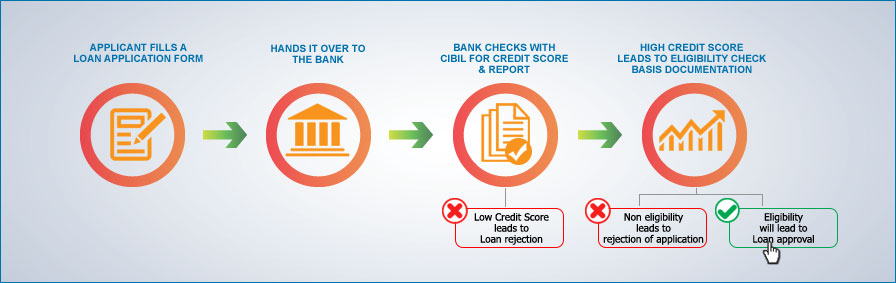
\includegraphics[width=\textwidth]{creditscoreflow.jpg}
\end{figure}

However, Credit Risk has recevied a lot of critisim as well from Academics and Researchers. \citep{al2002credit} has questioned about optimal method to evaulate customers? What are key variables or data points which an analyst must consider while evaulating customer applications? On what basis one can classify an applicant as good or bad?\\


However, apart from above questions following can be useful when building a new credit scoring system. One should evaluate statistical techniques or algorithm by its accuracy to correctly classify historical portfolios into good or bad credit from creditors file. Also, Banks and Financial institution's identified factors that can influence the prediction of credit and loan quality by gathering all possible information from customer applications form, bank transactions history and previous credit history. Credit Analysts analysis of all these information to decide what all variables or characteristics to be included in final the credit model.\\


One of the principal objectives of credit scoring system is to assist Banks and Financial Institutions to streamline their credit management procedure and policy that will enable analysts with an efficient tool which will provide fast and accurate analysis of credit.On the longer run, such tool helps banks to avoid bad credit and scale up bank revenues and profit by selling more financial products to customers.\\


Diffrrerent Technology in Credit Risk:\\

\textbf{Linear Regression}allows one to build to simple model using a dependent and two or more predictor data points, and it is being used in credit scoring models as the two class problems can be represented using a dummy variable \citep{lee2005two}. A Poisson regression can be used to classify cases where customer tends to partial repayments, and these payments can represent as a Poisson count in the model. Credit analysts can promptly analyse using linear regression credit model to investigate customer factor such as past payments record, credit guarantees and default, etc. against a predefined cut-off credit score. If new applicant credit score is higher than cut-off score, then credit is granted.\\

\textbf{Discriminant analysis} is a statistical analytics technique which most commonly used by research to analysis when two or more dependent variable is categorical, and the independent variable is interval scaled. Multiple Discriminant Analysis(MDA) utilised in various studies and business verticles for the variety of applications since its inception in 1930's \citep{fisher1936use}. \citet{durand1941risk} used the Discriminant analysis for modelling a scoring system that gives a prediction about loan repayment. Many researchers agreed that the MDA is the best use to classify a group of categorical variables into two or more predictor or classes. For example, Credit Analyst can build a scoring system using MDA to categorised a new loan application into Default or Non-Default category, and this will help banks to avoid those applicants who have potential to default in repayment sooner or later.\citet{altman1968financial} used MDA by developing a scoring model based on five financial ratios by analysing financial statements to select eight variables for predicting financial bankruptcy in Corporates. \citet{eisenbeis1978problems} noted the problem associated with Discriminant Analysis such as reduction in dimensionality, improper estimation of classification error, using linear functions instead of quadratic functions, etc.


Probit analysis


Decision trees

fdgdfh

Expert systems



Neural networks


Genetic programming was introduced by \citet{koza1992evolution} 



























Credit analysis and assessment is very important for banks and financial instituions to evaluate the credit worthiness of an applicant or a borrower. Banks implements various factors while assessing credit risk; such as credit rating, loan to value ratio, probability of default, etc.; that leads to derivation of credit risk rating. Variety of financial techniques have been used by the officials to analyse credit risk. 

\subsection{Examples of citations}\label{SS.citations}

In \citep{Atiyah:1961,Atiyah:1966a,Atiyah:1966b}, Atiyah builds on the work of \citet{Adams:1962} to develop 
the foundations of topological $K$-theory.  \citet{LewMcG:2000} and \citet{McG:2002} later extend parts of 
this to a previously unexplored algebraic setting.
